\documentclass{mwrep}
\usepackage{graphicx}
\usepackage[space]{grffile}
% Polskie znaki
\usepackage{polski}
\usepackage[utf8]{inputenc}
\usepackage[T1]{fontenc}
\usepackage{lmodern}
\usepackage{indentfirst}

% Strona tytułowa
\usepackage{pgfplots}
\usepackage{siunitx}
\usepackage{paracol}
\usepackage{gensymb}

% Pływające obrazki
\usepackage{float}
\usepackage{svg}
\usepackage{graphicx}

% table of contents refs
\usepackage{hyperref}
\usepackage{cleveref}
\usepackage{booktabs}
\usepackage{listings}
\usepackage{placeins}
\usepackage{xcolor}
\usepackage[left= 3cm, textwidth=10cm]{geometry}
\sisetup{detect-weight,exponent-product=\cdot,output-decimal-marker={,},per-mode=symbol,binary-units=true,range-phrase={-},range-units=single}
\SendSettingsToPgf
%konfiguracje pakietu listings
\lstset{
	backgroundcolor=\color{gray},
	frame=single,
	breaklines=true,
}
\lstdefinestyle{customlatex}{
	basicstyle=\footnotesize\ttfamily,
	%basicstyle=\small\ttfamily,
}
\lstdefinestyle{customc}{
	breaklines=true,
	frame=tb,
	language=C,
	xleftmargin=0pt,
	showstringspaces=false,
	basicstyle=\small\ttfamily,
	keywordstyle=\bfseries\color{green!40!black},
	commentstyle=\itshape\color{purple!40!black},
	identifierstyle=\color{blue},
	stringstyle=\color{orange},
}
\lstdefinestyle{custommatlab}{
	captionpos=t,
	breaklines=true,
	frame=tb,
	xleftmargin=0pt,
	language=matlab,
	showstringspaces=false,
	%basicstyle=\footnotesize\ttfamily,
	basicstyle=\scriptsize\ttfamily,
	keywordstyle=\bfseries\color{green!40!black},
	commentstyle=\itshape\color{purple!40!black},
	identifierstyle=\color{blue},
	stringstyle=\color{orange},
}

%wymiar tekstu 
\textwidth 160mm \textheight 247mm

%ustawienia pakietu pgfplots
\pgfplotsset{
tick label style={font=\scriptsize},
label style={font=\small},
legend style={font=\small},
title style={font=\small}
}

\def\figurename{Rys.}
\def\tablename{Tab.}

%konfiguracja liczby 
\setcounter{topnumber}{0}%2
\setcounter{bottomnumber}{3}%1
\setcounter{totalnumber}{5}%3
\renewcommand{\textfraction}{0.01}%0.2
\renewcommand{\topfraction}{0.95}%0.7
\renewcommand{\bottomfraction}{0.95}%0.3
\renewcommand{\floatpagefraction}{0.35}%0.5

\begin{document}
\frenchspacing
\pagestyle{uheadings}

%strona 
\title{\bf Sprawozdanie z projektu i ćwiczenia laboratoryjnego nr 1, zadanie nr 4\vskip 0.1cm}
\author{Piotr Chachuła, Cezary Dudkiewicz, Piotr Roszkowski}
\date{2019}

\makeatletter
\renewcommand{\maketitle}{\begin{titlepage}
\begin{center}{\LARGE {\bf
Wydział Elektroniki i Technik Informacyjnych}}\\
\vspace{0.4cm}
{\LARGE {\bf Politechnika Warszawska}}\\
\vspace{0.3cm}
\end{center}
\vspace{5cm}
\begin{center}
{\bf \LARGE Projektowanie układów sterowania\\ (projekt grupowy) \vskip 0.1cm}
\end{center}
\vspace{1cm}
\begin{center}
{\bf \LARGE \@title}
\end{center}
\vspace{2cm}
\begin{center}
{\bf \Large \@author \par}
\end{center}
\vspace*{\stretch{6}}
\begin{center}
\bf{\large{Warszawa, \@date\vskip 0.1cm}}
\end{center}
\end{titlepage}
}
\makeatother

\maketitle

\tableofcontents
\part{Projekt}
\label{PROJEKT}
\chapter{Weryfikacja punktu pracy}
\label{zad1}

\section{Opis postępowania}
\label{zad1_opis}
W celu sprawdzenia poprawności wartości sygnałów $u$, $y$ oraz $z$ pobudzono obiekt sterowaniem
o wartości $u = \num{0.0}$, zakłóceniem $z = \num{0.0}$ i sprawdzeniu czy stabilizuje się on w punkcjie pracy  $y = \num{0.0}$. Do symulacji wyjscia obiektu użyto udostępnionej funkcji 
\verb+symulacja_obiektu4y.+ Do testów napisano skrypt \verb+Zad1.m. + Wyniki przedstawiono poniżej.

\section{Wyniki}
\label{zad1_wyniki}
Zgodnie z przewidywaniami wyjscie obiektu ustaliło się na wartości $y= \num{0.0}$. Punkt pracy ustalony jest więc poprawnie.
\begin{figure}[tb]
	\centering
	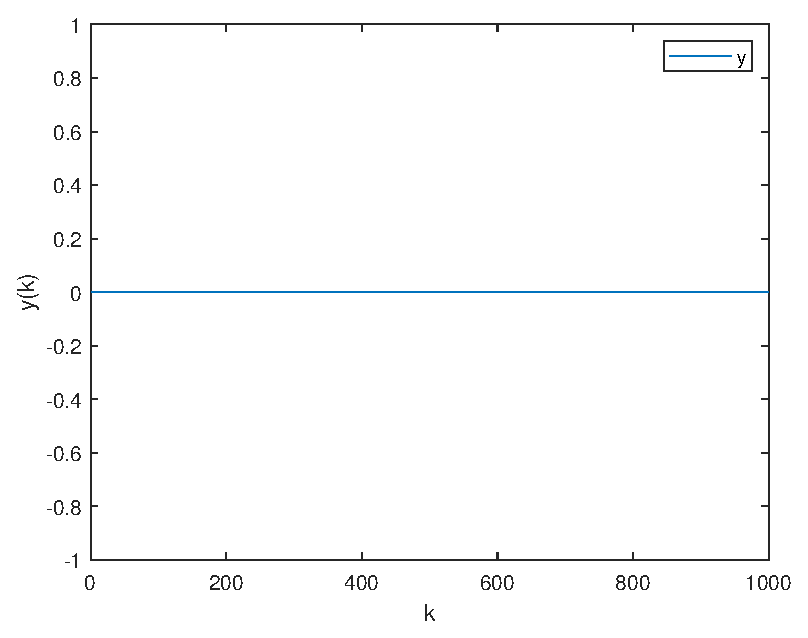
\includegraphics[scale=1]{Rys/punkt_pracy.eps}
	%\includegraphics[scale=1]{rysunki/zapisz_pdf/symulacje11}
	\caption{Odpowiedź obiektu na sterowaniei $u=\num{0.0}$ i zakłócenie $z = \num{0.0}$}
\end{figure}
\chapter{Odpowiedzi skokowe}
\label{zad2}

\section{Wyznaczanie odpowiedzi skokwych}
\label{zad2_skoki}

\begin{figure}[t]
\centering
    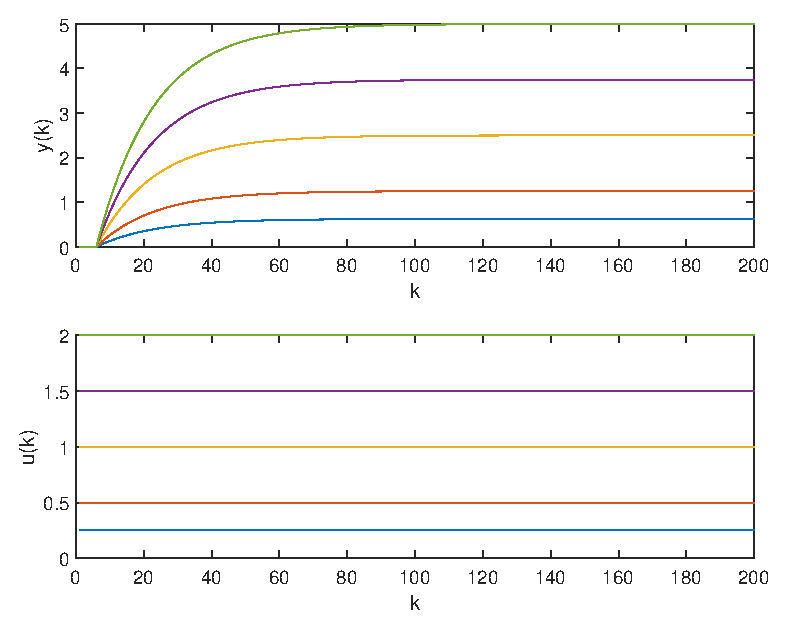
\includegraphics[scale=1]{Rys/odp_skok_u.eps}
    \caption{Odpowiedz procesu na skokową zmiane sterowania}
    \label{zad2_odp_skok_u}
\end{figure}

\begin{figure}[t]
	\centering
	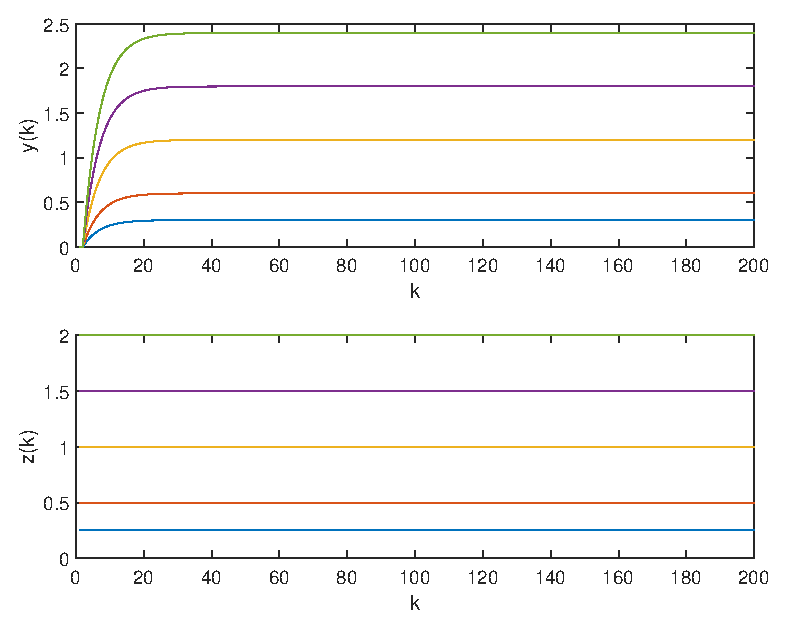
\includegraphics[scale=1]{Rys/odp_skok_z.eps}
	\caption{Odpowiedz procesu na skokową zmiane zakłócenia}
	\label{zad2_odp_skok_z}
\end{figure}

W celu wyznaczenia odpowiedzi skokowej obiekt, znajdujący się w punkcie pracy (tzn. $u= \num{0.0}$, $z= \num{0.0}$, $y= \num{0.0}$) pobudzony zostaje skokową wartością sterowania/zakłócenia. Rysunek \ref{zad2_odp_skok_u} oraz \ref{zad2_odp_skok_z} przedstawia odpowiedź obiektu na dane skoki.

\section{Wyznaczanie charakterystyki statycznej procesu}
\label{zad2_char_stat}
Aby wyznaczyć charakterystykę statyczną procesu przeprowadzono analogiczne działania co w rozdziale \ref{zad1}. Tym razem przy użyciu skryptu \verb+Zad2.m +dla wielu wartosci $u$ oraz $z$ wyznaczono odpowiadające im $y$ oraz z ich pomocą utworzono wykres \ref{zad2_char_stat}. Jak widać charakterystyka statyczna obiektu jest liniowa, a co za tym idzie obiekt jest liniowy.

\begin{figure}[b]   
     \label{zad2_char_stat}
    \centering
    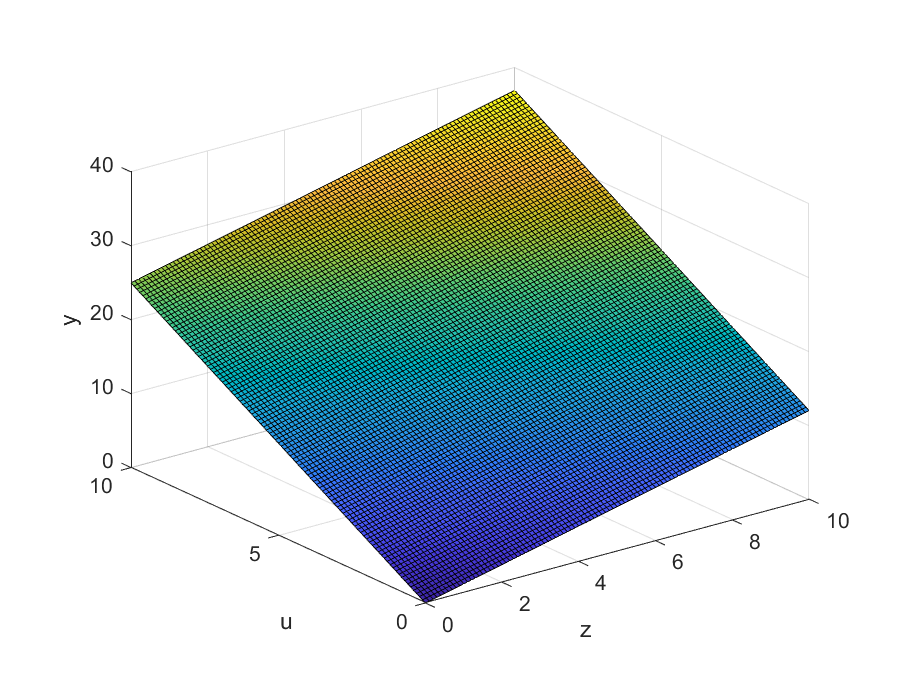
\includegraphics[scale=1]{Rys/char_stat.eps}
    \caption{Charakterystka statyczna $y(u,z)$ symulowanego procesu}

\end{figure}

\section{Wzmocnienie statyczne}
\label{zad2_wzmocnienie}
Wzmocnienie statyczne, czyli stosunek pomiędzy zmianą wartosci wyjscia i zmianą wartosci wejścia w stanie ustalonym. Aby ją wyznaczyć można na przykład znaleźć nachylenie charakterystyki statycznej do osi OU lub OZ, czyli np.:

\begin{equation}
K_{\mathrm{stat}_u} = \frac{y(u_{\mathrm{max}})- y(u_{\mathrm{min}})}{u_{\mathrm{max}}- u_{\mathrm{min}}}
\label{zad2_wzm_statyczne_wzor}
\end{equation}

W przypadku tak wykreślonej charakterystyki, wzmocnienie statyczne jest równe tangensowi kąta $\alpha$
pomiędzy prostą a osią $OU$. 
\begin{equation}
K_{\mathrm{stat}_u} = \frac{24.9903- 0}{10- 0}\approx 2.5
\label{zad2_wzm_statyczne_u}
\end{equation}
\begin{equation}
K_{\mathrm{stat}_z} = \frac{11.9884- 0}{10- 0}\approx 1.2
\label{zad2_wzm_statyczne_z}
\end{equation}

\chapter{Wyznaczanie odpowiedzi skokowych}
Odpowiedz skokowa w algorytmie DMC oznacza odpowiedz obiektu na jednostkowy skok sterowania. Wyznacza się ją poprzez albo pobudzenie obiektu takim właśnie skokiem jednostkowym, albo, gdy jest to niemożliwe, jakimkolwiek innym i normalizowanie jej. W naszym przypadku nic nie stoi na przeszkodzie aby odrazu pobudzić obiekt takimi właśnie sygnałami.

\begin{figure}[h!]
	\centering
	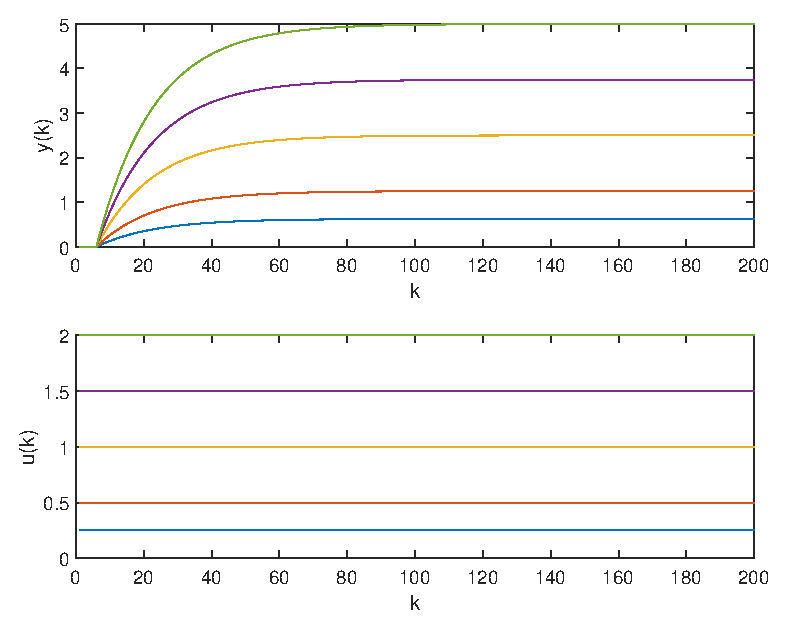
\includegraphics[scale=1]{Rys/odp_skok_u.eps}
	\caption{Odpowiedz skokowa obiektu pobodzonego jednotkowym skokiem sterowania$u$}
	\label{Rys:odp_skok_u}
\end{figure}
\begin{figure}[h!]
	\centering
	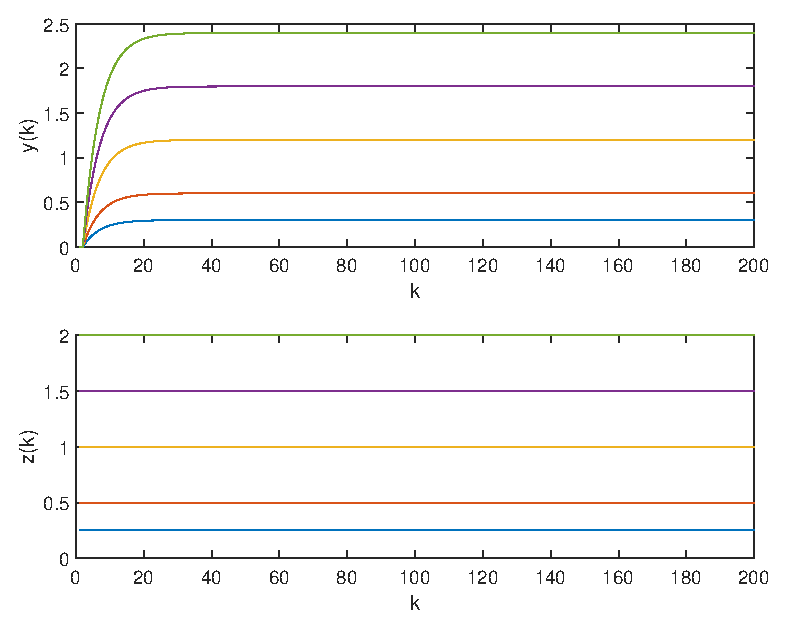
\includegraphics[scale=1]{Rys/odp_skok_z.eps}
	\caption{Odpowiedz skokowa obiektu pobodzonego jednotkowym skokiem sterowania$z$}
	\label{Rys:odp_skok_z}
\end{figure}
\chapter{Regulator DMC}
\label{zad4}


\section{Algorytm działania}
Algorytm działania regulatora oraz implementacja została dobrze udokumentowana w pliku \verb+DMC_Z.m +. Listing jego częsci algorytmicznej przedstawiony jest poniżej:
\begin{lstlisting}[style=custommatlab,frame=single,label={zad4_sim_lst},caption={Implementacja regulatora DMC},captionpos=b]

function [Err] = DMC_Z (paras)
% zmienne i macierze regulatora
load('odp_skok');
D=paras(1);
N = paras(2);
Nu=paras(3);
lambda = paras(4);
DZ = 25;
s = su;
z = zeros(N,1);
z(1:size(sz))=sz;
z(size(sz):end)=sz(end);

M=zeros(N,Nu);
for i=1:N
for j=1:Nu
if (i>=j)
M(i,j)=s(i-j+1);
end
end
end

MP=zeros(N,D-1);
for i=1:N
for j=1:D-1
if i+j<=D
MP(i,j)=s(i+j)-s(j);
else
MP(i,j)=s(D)-s(j);
end    
end
end

MZP=zeros(N,DZ);
for i=1:N
MZP(i,1) = z(i);
for j=2:DZ
if i+j-1<=DZ
MZP(i,j)=z(i+j-1)-z(j);
else
MZP(i,j)=z(DZ)-z(j);
end      
end
end

I=eye(Nu);
K=((M'*M+lambda*I)^-1)*M';
ku=K(1,:)*MP;
kz=K(1,:)*MZP;
ke=sum(K(1,:));
deltaup=zeros(1,D-1);
deltazp=zeros(1,DZ-1);

% dane
n = 200;
U0 = 0;
Z0 = 0;
Y0 = 0;
start = 10;

U = U0*ones(1,n);
Z = Z0*ones(1,n);
Z(100:end) = 1;
Y = Y0*ones(1,n);
Yz = Y;
Yz(10:end) = 1;
e = zeros(1,n);

%hold on
for k = start:n
Y(k) = symulacja_obiektu4y(U(k-6),U(k-7),Z(k-2),Z(k-3),Y(k-1),Y(k-2));
e(k) = Yz(k) - Y(k);

%uwzglednianie zaklocenia
for i = DZ:-1:2
deltazp(i) = deltazp(i-1);
end
deltazp(1) = Z(k) - Z(k-1);

% Prawo regulacji
deltauk = ke*e(k)-ku*deltaup'-kz*deltazp';

for i = D-1:-1:2
deltaup(i) = deltaup(i-1);
end
deltaup(1) = deltauk;
U(k) = U(k-1)+deltaup(1);
end
Err = (Yz-Y)*(Yz-Y)';
end

\end{lstlisting}


\section{Strojenie regulatora DMC}


Strojenie regulatora przeprowadzone zostało metodą automatyczną przy użyciu\\ funkcji \verb+ga(@DMC,nvars,[],[],[],[],lb,ub,[],IntCon,options)+. Strojonymi parametrami były $N$, $N_u$ oraz $\lambda$. Za dolne ograniczenie przyjęte zostały wartości $N=1$, $N_u = 1$, $\lambda = 1$, natomiast za górne $N=D$, $N_u = D$ oraz $\lambda = 1000$, gdzie $D = 116$. Wyniki strojenia regulatora przedstiowone są na wykresie \ref{fig:strojenie}.

\begin{figure}[h!]
	\centering
	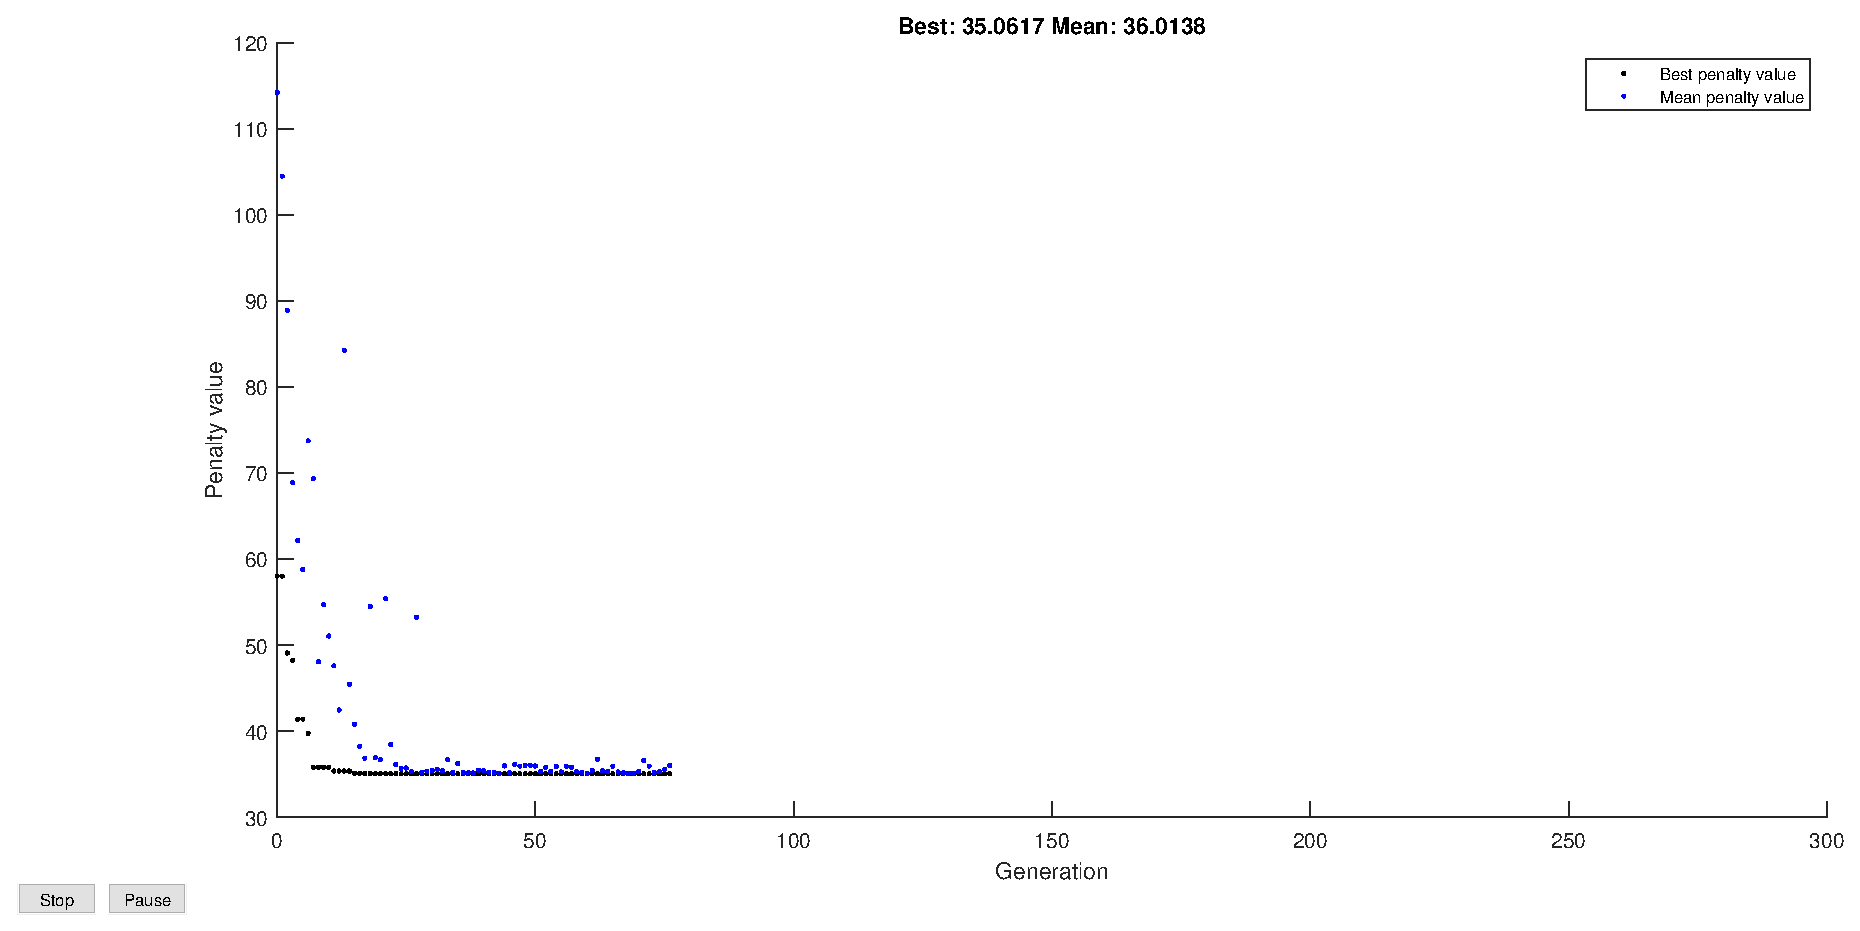
\includegraphics[scale=0.5]{Rys/strojenie.eps}
	\caption{Wyniki strojenia regulatora przy użyciu funkcji $ga$}
	\label{fig:strojenie}
\end{figure}

Przykładowy przebieg pokazujący pracę wystrojonego już regulatora można zobaczyć na wykresie \ref{fig:przebieg1}

\begin{figure}
	\centering
	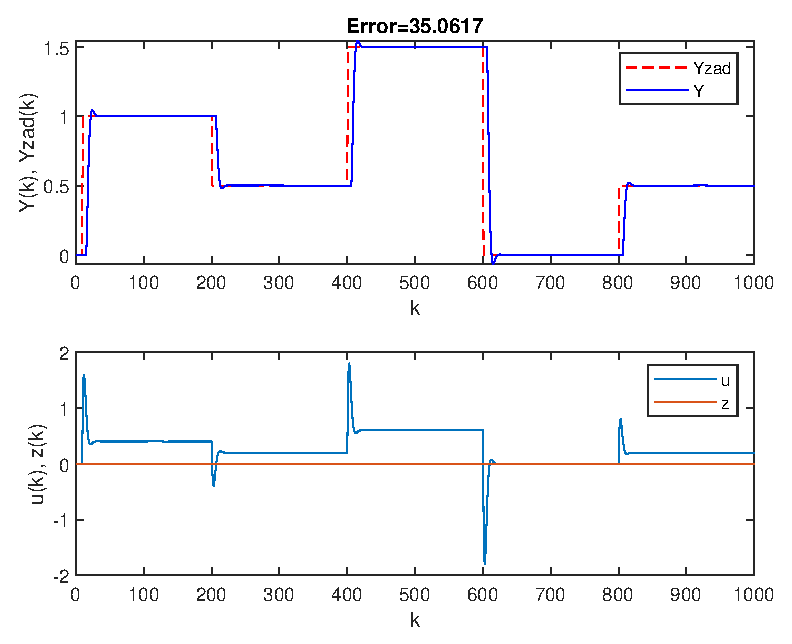
\includegraphics[scale=1]{Rys/przebieg1.eps}
	\caption{Przebieg dla parametrów $N = 116$, $N_u = 4$, $\lambda = 1$}
	\label{fig:przebieg1}
\end{figure}

\chapter{Zakłócenie w regulatorze DMC}
\label{zad5}
Poniżej (rys. \ref{fig:zak_bezr}) został zaprezentowany przebieg, w którym po osiągnięciu wartości zadanej, w chwili $k=100$ następuje skokowy wzrost zakłócenie z $0$ na $1$.

\begin{figure}[h!]
	\centering
	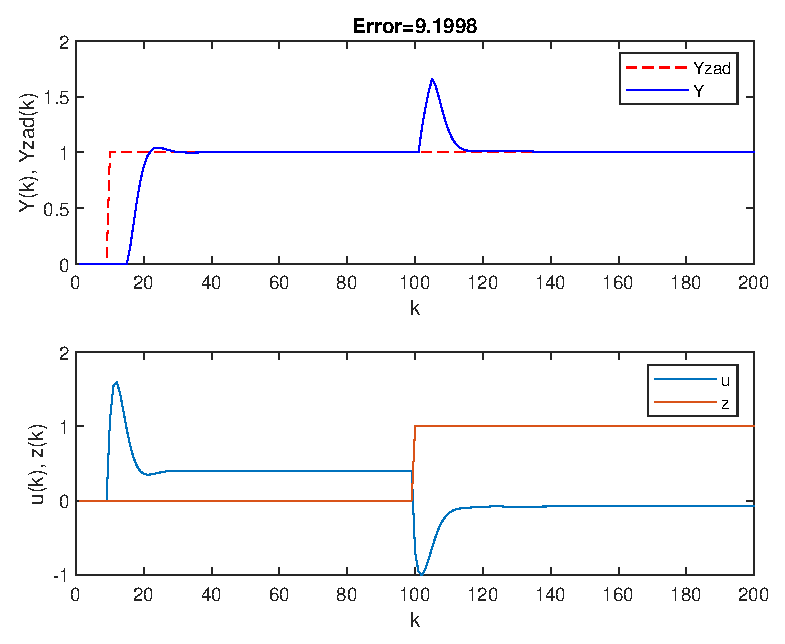
\includegraphics[scale=1]{Rys/zak_bezr.eps}
	\caption{Przebieg bez uwzględniania zakłócenia w regulacji}
	\label{fig:zak_bezr}
\end{figure}

\section{Dobór parametru $D_z$}
Prametr $D_z$ został dobrany, podobniej jak inne, za pomącą funkcji \verb|ga|. Poszykiwanie zostało przedstawione na wykresie \ref{fig:stojenie_dz}.

\begin{figure}[h!]
	\centering
	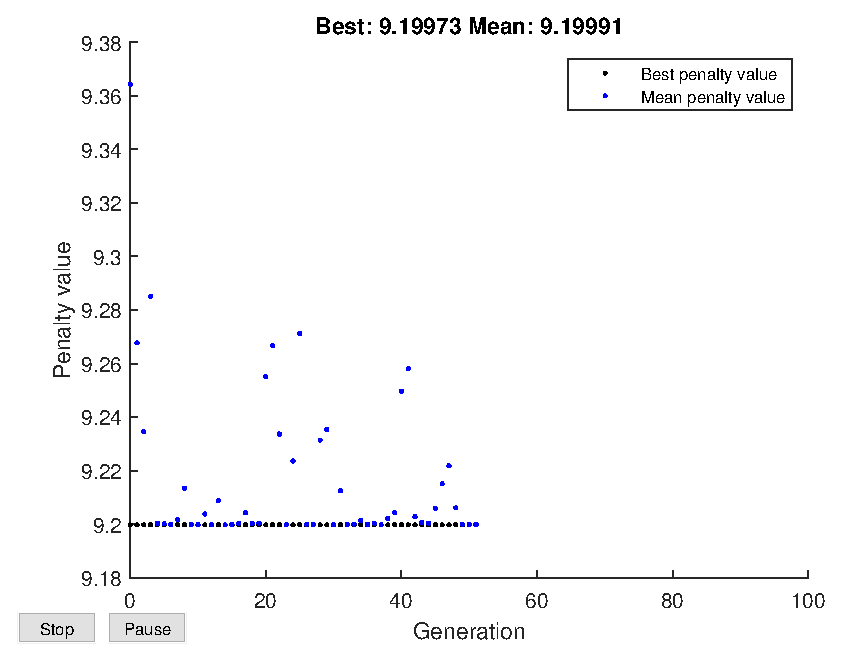
\includegraphics[scale=1]{Rys/strojenie_dz.eps}
	\caption{Poszukiwanie parametru $D_z$}
	\label{fig:stojenie_dz}
\end{figure}

Najlepszą jakość regulacji osiągnięto dla $D_z = 25$. Przebieg dla tej wartości można zobaczyć na wykresie \ref{fig:zak_zr}

\begin{figure}[h!]
	\centering
	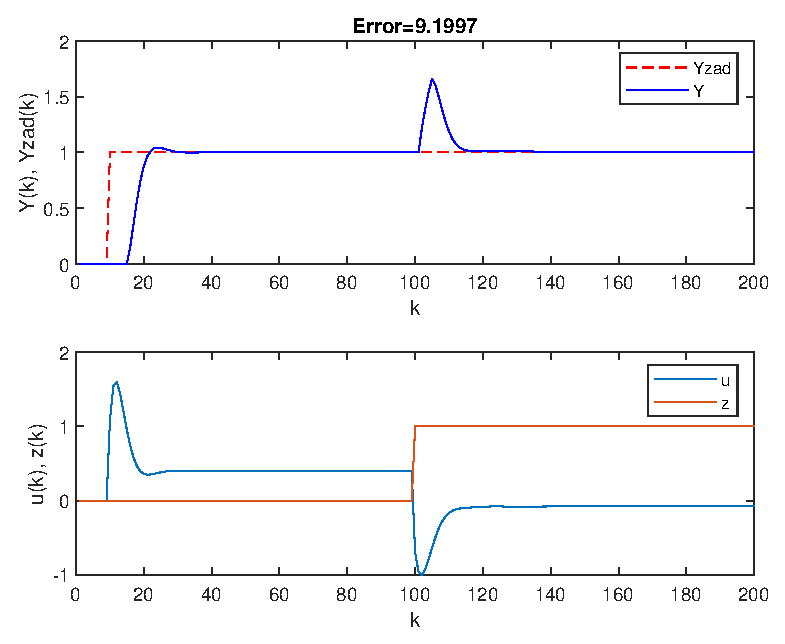
\includegraphics[scale=1]{Rys/zak_zr.eps}
	\caption{Przebieg z uwzględnieniem zakłócenia w regulacji}
	\label{fig:zak_zr}
\end{figure}

\FloatBarrier

\section{Omówienie wyników}
Jak można zaobserwować na wykresach \ref{fig:zak_bezr} i \ref{fig:zak_zr} regulator biorący pod uwagę zakłócenie znacznie lepiej radzi sobie z zakłóceniem, szybciej wraca do wartości zadanej i zapobiega większym błędom.
\chapter{Zakłócenie sinusoidalne}
W celu sprawdzenia wpływu zakłócenia sinusoidalnego na jakość regulacji (z pomierem i bez pomiaru) wygenerowane zostały przebiegi z zakłóceniami o różnej częstotliwości i różnej amplitudzie. Sygnałem zakłócający generowany był jako
\begin{equation}
	z = sin(k/p)*a
	\label{eq:zaksin}
\end{equation}
gdzie $p$ przybierało wartości:
\begin{itemize}
	\item $p=5$,
	\item $p=10$,
	\item $p=20$,
\end{itemize}
natomist $a$:
\begin{itemize}
	\item $a=0.1$,
	\item $a=0.2$,
	\item $a=1$.
\end{itemize}
Tak przygotowane wykresy można obejrzeć poniżej.
\begin{figure}[h!]
	\centering
	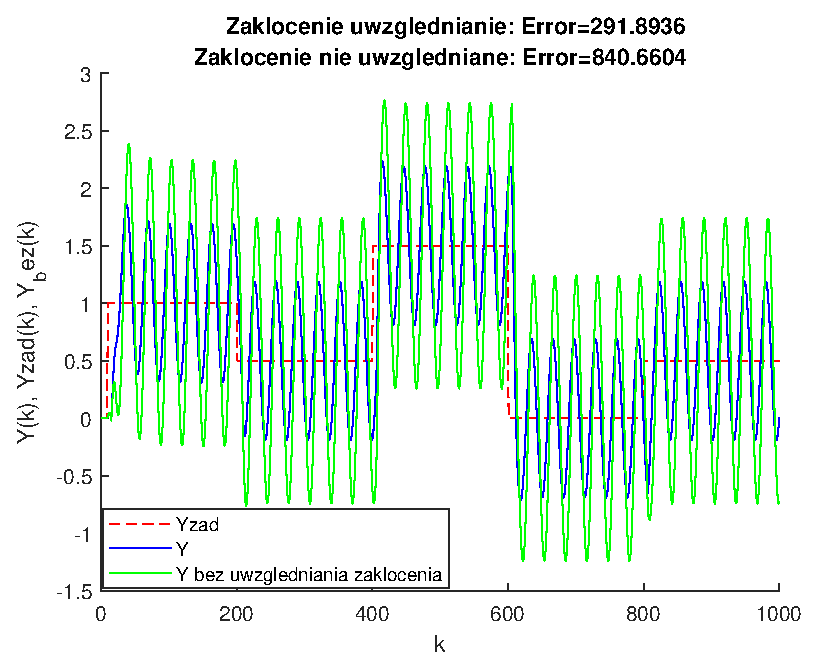
\includegraphics[scale=1]{Rys/sin5_1}
	\label{fig:sin5_1}
	\caption{Przebieg dla zakłócenia z parametrami $p=5$ oraz $a=1$}
\end{figure}
\begin{figure}[h!]
	\centering
	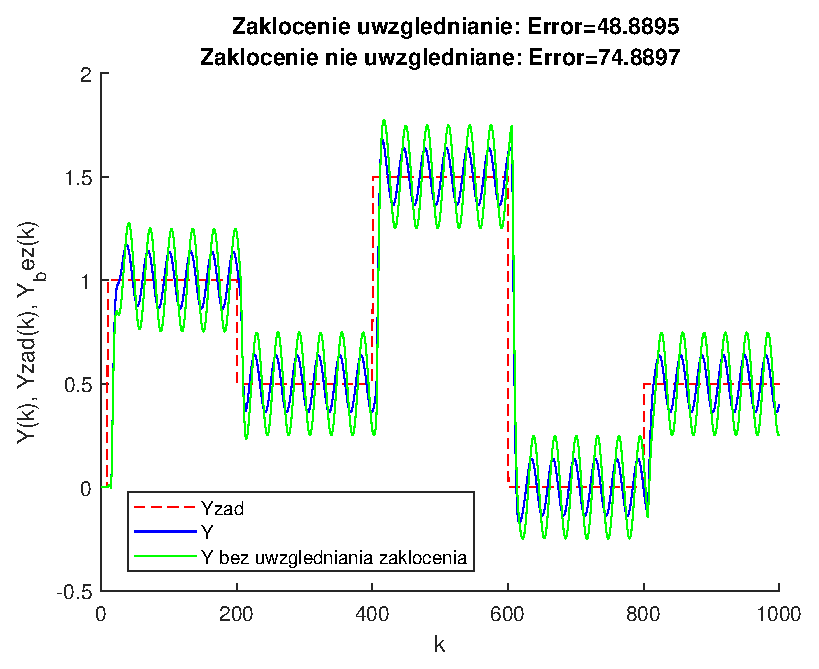
\includegraphics[scale=1]{Rys/sin5_5}
	\label{fig:sin5_5}
	\caption{Przebieg dla zakłócenia z parametrami $p=5$ oraz $a=0.2$}
\end{figure}
\begin{figure}[h!]
	\centering
	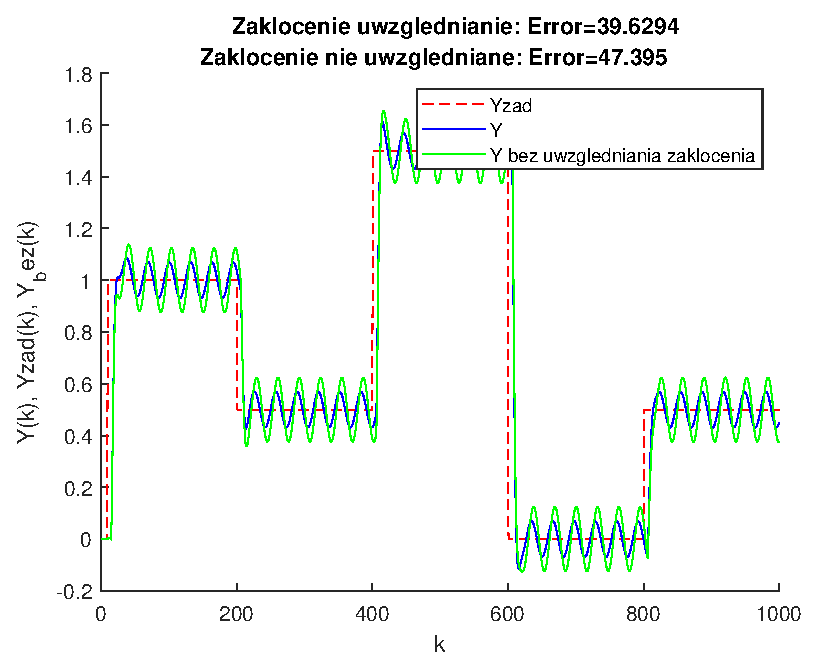
\includegraphics[scale=1]{Rys/sin5_10}
	\label{fig:sin5_10}
	\caption{Przebieg dla zakłócenia z parametrami $p=5$ oraz $a=0.1$}
\end{figure}
\begin{figure}[h!]
	\centering
	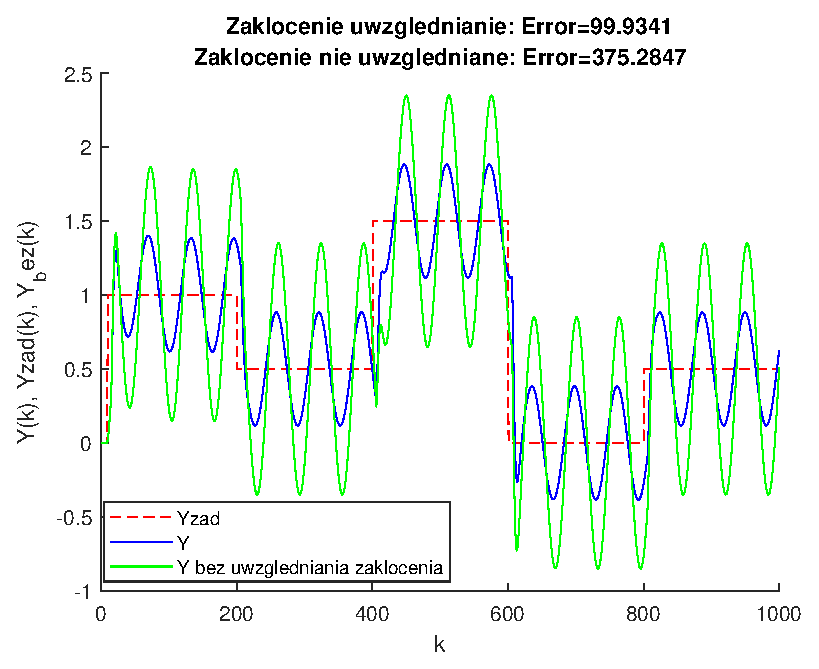
\includegraphics[scale=1]{Rys/sin10_1}
	\label{fig:sin10_1}
	\caption{Przebieg dla zakłócenia z parametrami $p=10$ oraz $a=1$}
\end{figure}
\begin{figure}[h!]
	\centering
	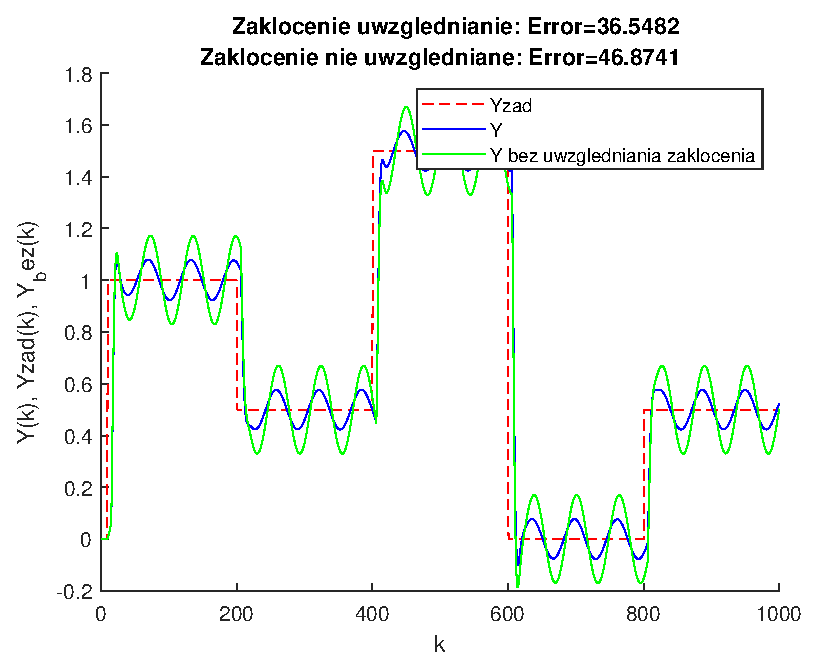
\includegraphics[scale=1]{Rys/sin10_5}
	\label{fig:sin10_5}
	\caption{Przebieg dla zakłócenia z parametrami $p=10$ oraz $a=0.2$}
\end{figure}
\begin{figure}[h!]
	\centering
	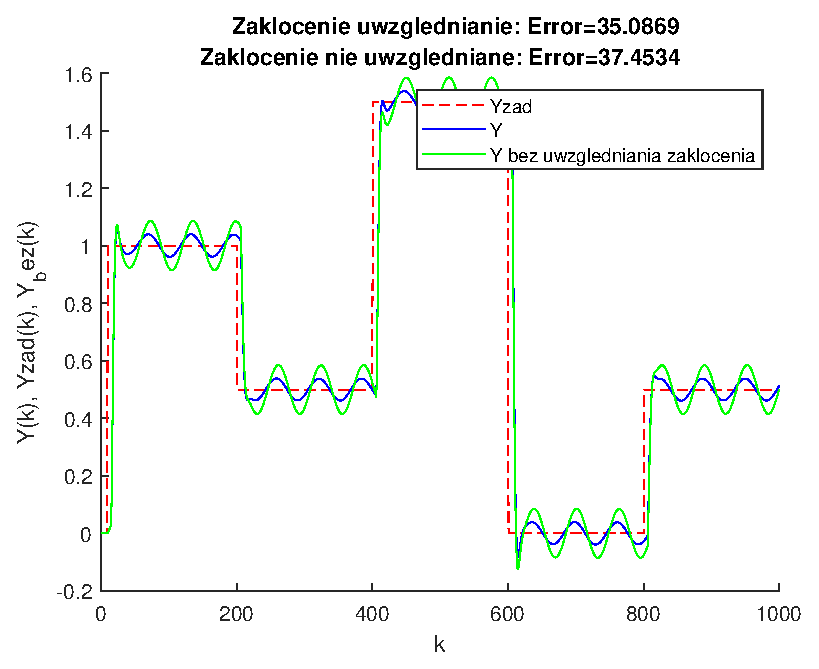
\includegraphics[scale=1]{Rys/sin10_10}
	\label{fig:sin10_10}
	\caption{Przebieg dla zakłócenia z parametrami $p=10$ oraz $a=0.1$}
\end{figure}
\begin{figure}[h!]
	\centering
	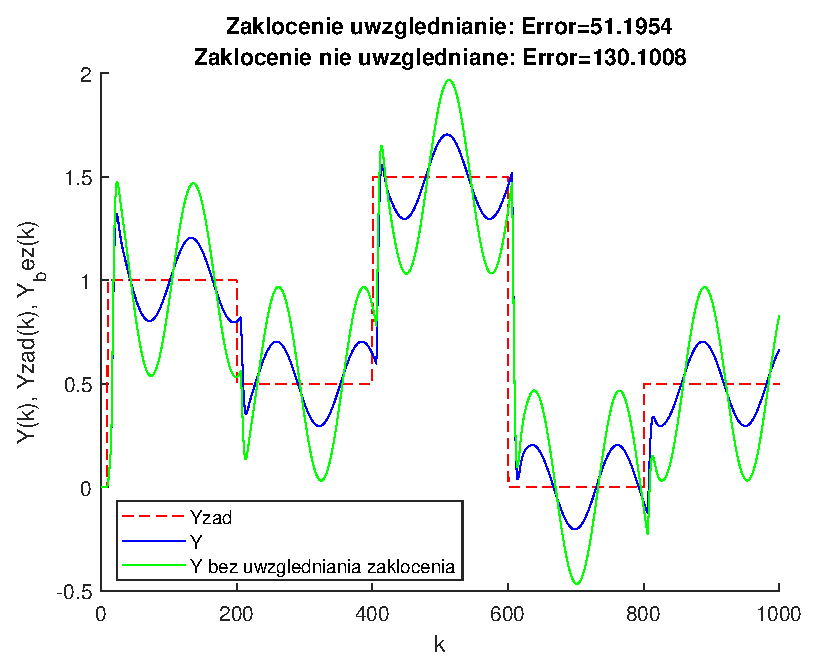
\includegraphics[scale=1]{Rys/sin20_1}
	\label{fig:sin20_1}
	\caption{Przebieg dla zakłócenia z parametrami $p=20$ oraz $a=1$}
\end{figure}
\begin{figure}[h!]
	\centering
	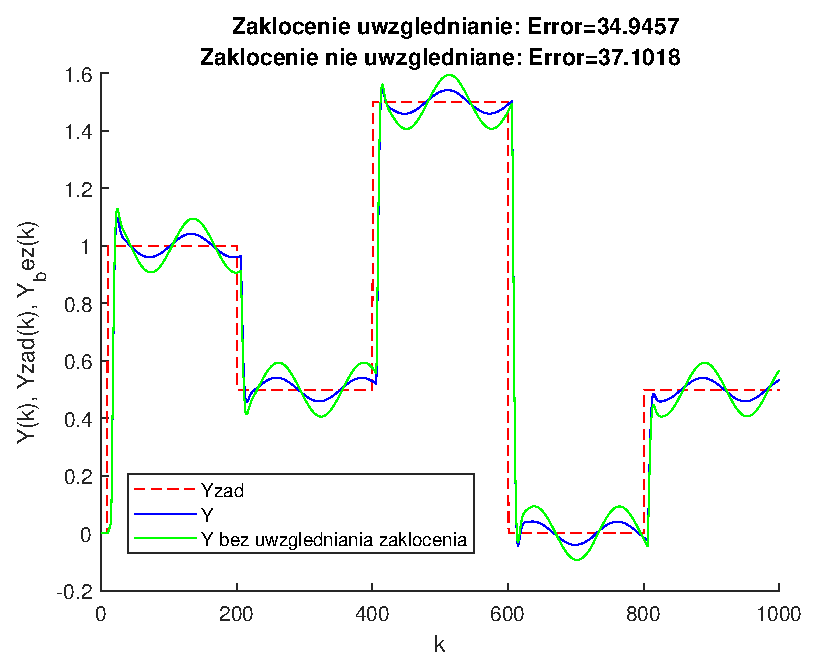
\includegraphics[scale=1]{Rys/sin20_5}
	\label{fig:sin20_5}
	\caption{Przebieg dla zakłócenia z parametrami $p=20$ oraz $a=0.2$}
\end{figure}
\begin{figure}[h!]
	\centering
	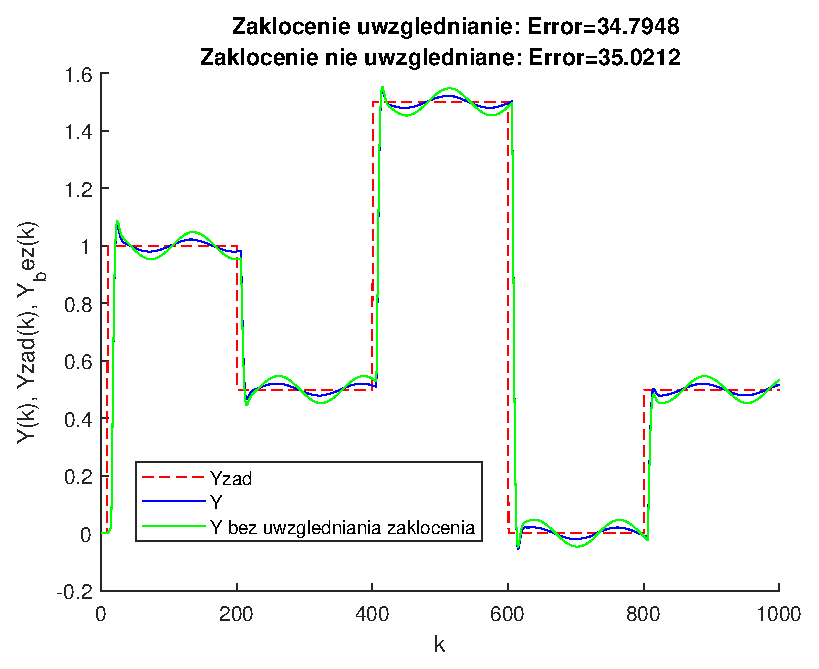
\includegraphics[scale=1]{Rys/sin20_10}
	\label{fig:sin20_10}
	\caption{Przebieg dla zakłócenia z parametrami $p=20$ oraz $a=0.1$}
\end{figure}

\part{Laboratoria}


\appendix
\end{document}